\subsection{General reset}
\label{sec:GENERAL_RESET}

Once the \textbf{\textit{Open}}/\textbf{\textit{Error}} message has been displayed for a few ms, all programmable logic devices must be reset.
\medskip

In order to do this, the \emph{RESET} signal that commands all the GALs, is operated with \emph{ENDPULSE\_SEND} output. This signal can come from two GALs, the \emph{OPEN} and the \emph{ERROR} one, and it indicates when the cycle is over, i.e. when the Open/Error message has been displayed for a few ms and the status LED has either turned red or green. To save some money and space, both of these signals have been connected to an OR gate which output is fed directly into one of the timers mentioned in \textbf{Subsubsection \ref{sec:DELAYED_PULSE}}. The timer's output is connected to the \emph{RESET}, which resets all the state machines.

\begin{figure}[H]
    \centering
    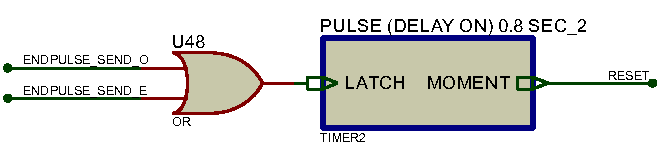
\includegraphics[scale = 1]{Graphics/GENERAL RESET/GENERAL_RESET.PDF}
    \caption{General Reset Proteus Subassembly}
    \label{fig:GENERAL_RESET}
\end{figure}{}